\chapter{GEM detectors }\label{ch:gem}

\section{Introduction}
%\section{Introduction}
As a particle physicist, we need to understand the properties of particles, how it interact with other matter. %But for that we need a sophisticated detector that can detect, track, and/or identify high-energy particles produced in a particle accelerator. We also need to measure the energy, momentum, spin, charge, etc of the particles.
In order to understand the nature we need to develop and use technically sophisticated tools like various detectors, accelerators, etc.
%From the early scattering experiment of Rutherford to the colliding beam experiments that produced the top quark with a mass almost as large as Rutherford's gold nucleus, particle beams have been the mainstay of elementary particle physics. Elementary particle physicists are motivated to develop and use technically sophisticated tools by a deep desire to understand how the world works and its most basic and fundamental level. 
The best particle detectors in the world is situated at the LHC. %There are mainly four hermetic detectors, namely, \gls{cms}, \gls{atlas}, \gls{alice}, \gls{lhcb}. Our work is based on the upgradation of the one of detectors in \gls{cms} namely, \gls{gem}.

The LHC is designed to collide protons at a frequency of 40MHz. We do not yet have the technology to handle and store all the produced data at this rate. Inside the {cms}, one of the four {lhc}'s experiment, each event produces approximately 1 Megabytes of analyzed data, while the detector generates several Terabytes every second. The maximum amount of data that CMS can store every day is of the order of the Terabytes, yielding a rate of accepted events of 100Hz, requiring the total rate to be divided by a factor of $4\times 10^5$.

This requires the installation of a trigger system which selects events of interest and handles data in real-time, coupled with a complex data acquisition system. The first stage of the {cms}'s trigger system, called the Level1 Trigger (L1 Trigger), analyzes the information from the calorimeters and the muon chambers, using algorithms programmed on dedicated electronics, and performs a first selection of interesting events. It is important to ensure that the system has the capability to recognize the signature of interesting physical processes, while rejecting the other $\sim 99.99975\%$ of the events.

The forward region of the CMS muon spectrometer is equipped with two different technologies of gaseous detectors: {csc} which yield a good spatial resolution of the order of $100\mu m$ and a time resolution of 5ns, and a {rpc} which offer a lower spatial resolution around 1mm but an excellent time resolution down to 1ns. In the most forward region of {cms}, the {rpc}s have not been installed and the L1 Trigger relies on {csc}s only. Currently, {cms} has the least redundancy, trigger capability, and reconstruction efficiency in the most challenging region for muon detection. High background fluxes and shorter tracks in the transverse plane constitute a challenge when trying to identify muons.

The presence of muons in the final state is a signature of many interesting processes such as the decay of the Higgs boson or new physics like super-symmetry. High energy muons often constitute the golden channel due to their high detection and reconstruction efficiency. At higher luminosity at which the {lhc} will run after Long-Shutdown 2 (LS2), the selection of muons will suffer from an increased background generating coincidence in the detectors and confusing the trigger. With only breadcrumbs of data available, the efficiency of the L1 Trigger will quickly diminish, degrading the performance of the {cms} muon spectrometer.

The standard {rpc}s are not designed to operate at the high rates of particle that will be reached after LS2 and will loose efficiency. New {gem} detectors already used in other experiments present the opportunity to equip the vacant region with detectors that have proven to maintain a spatial resolution of the order of $100\mu m$, a time resolution below 5 ns, and a detection efficiency above $98\%$  even at elevated fluxes. The objective of the {cms} {gem} collaboration is to instrument the most forward region of the {cms} muon spectrometer with Triple-{gem} detectors during LS2 \cite{phdThesis:Lenzi}.
\begin{comment}
\subsection{Introduction to CMS Detector}
The \gls{cms} is a general-purpose detector at the \gls{lhc}. It is very compact, high hermeticity and emphasizes good muon identification, good charge particle momentum resolution including efficient b and $\tau$ tagging capabilities as well as good electromagnetic energy resolution and a good missing transverse energy and dijet-mass resolution. It is designed to investigate a wide range of physics, including the search for the Higgs boson, extra dimensions, and particles that could make up dark matter. Furthermore, there are high hopes for discoveries that could pave the way toward a unified theory.  \gls{cms} is 25 meters long, 15 meters in diameter, and weighs about 14,000 tonnes. It is located in an underground cavern at Cessy in France, just across the border from Geneva.

The detector consists of several layers of sub-detectors and is organized in a barrel region, which is cylindrically shaped around the beam axis, and two endcap regions, disks closing the barrel region at both sides. The sub-detectors are situated in an onion-shell arrangement. The central system, a three barrel layer two forward disk pixel detector, is mainly responsible for b- and $\tau$-tagging as well as track seeding and primary vertex identification. It is followed by a 10 layer 12 forward disk silicon strip system, the main tracking device to determine momentum and energy and also to deal with the high track multiplicity. 


There are different sub-detector systems in the \gls{cms}. The role of each system in the reconstruction and identification of muons, electrons, charged and neutral hadrons and photons emerging from the interaction point is illustrated in Figure %\ref{cms}. 

\subsubsection{Magnet system}
To enable the measurement of the momenta of charged particles traversing \gls{cms}, their trajectories are bend by the magnetic field produced by the \gls{cms} solenoid. This superconducting solenoid encompasses a cylindrical volume, 12.5m in length and 6m in diameter centered around the interaction point. Inside this volume, the magnet produces a uniform 3.8T magnetic field. Outside the solenoid, most of the magnetic flux
\end{comment}

\chapter{Gas Electron Multiplier}
%\section{Introduction}
{gem} is a new idea from Fabio Sauli at CERN \cite{paper:NIMPR:FSauli}. Developed as a way of boosting the performance of microstrip gas chambers. The objective is to match the harsh running conditions of experiments at CERN's LHC collider, where detectors will have to cope with high data rates and will be exposed to intense bombardment by high-energy particles \cite{article:cernCourier:gem}.

{gem} is a thin sheet of plastic coated with metal on both sides and chemically pierced by a regular array of holes a fraction of a millimeter across and apart. Applying a voltage (about 500V on 50$\mu$) across the {gem} conducting layers, the resulting high electric field in the holes makes an avalanche of ions and electrons pour through each. The {gem} foil is shown in Figure \ref{gem}.
\begin{figure}[htb]
	\begin{center}
		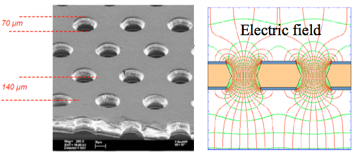
\includegraphics[width=12.0cm,height=5cm]{figures/GEM/KEKDTP3.jpg}
		\caption{(Left) The gas electron multiplier (GEM) foil can image two-dimensional position of particles passing through a gaseous chamber. (Right) The cross sectional view of the GEM shows strong electric fields in the vicinity of holes where electron signals are amplified.}
		\label{gem}
	\end{center}
\end{figure} 

The region inside {gem} detector consists of a drift electrode, a conversion and drift region, a {gem} mesh collecting and multiplying the charge in a gas avalanche, and induction gap in which a high electric field is used to extract and drift the electrons towards the collecting electrodes. This is shown in Figure \ref{gemgaps}. The large effective gains (up to $10^4$), full efficiency of detection and very good localization accuracies for minimum ionizing particles is promissing to us. In the thin gap of {gem} few tens of primary ion pairs creates; cascading to two {gem} meshes so it can provide large gains and better performances \cite{paper:2dgem}.
\begin{figure}[htb]
	\begin{center}
		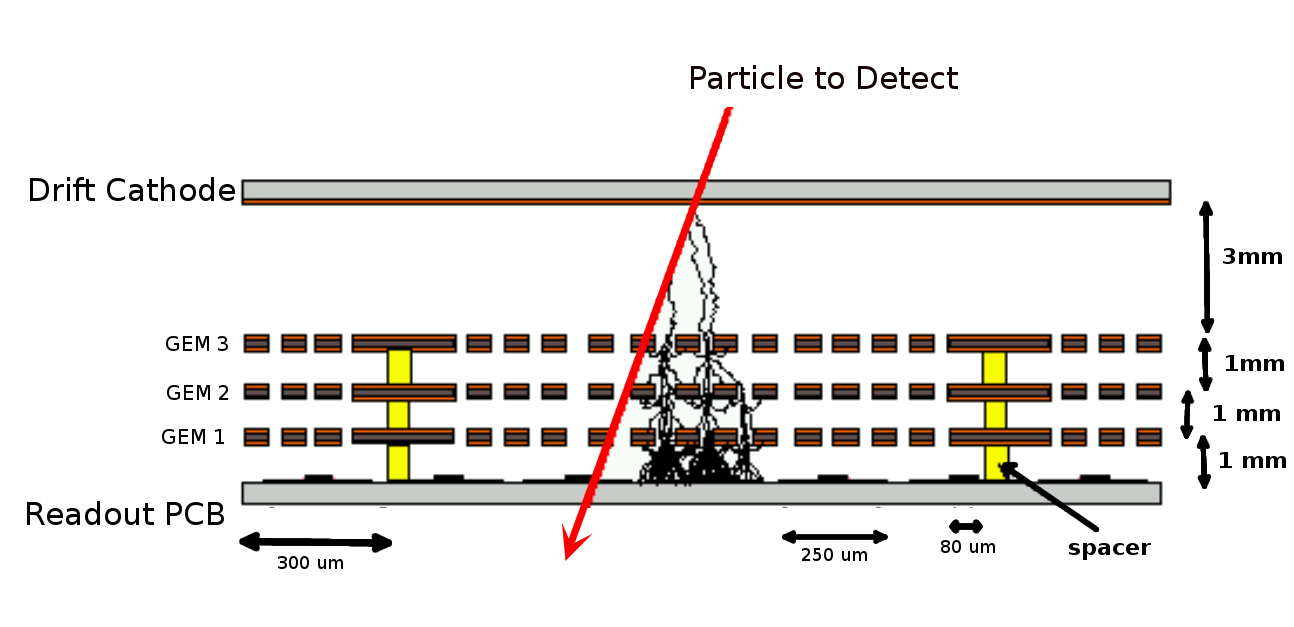
\includegraphics[width=10.0cm,height=7cm]{figures/GEM/triple_gem.png}
		\caption{Illustration of GEM working}
		\label{gemgaps}
	\end{center}
\end{figure} 

\section{GEM for CMS}
The CMS experiment was designed to have a highly redundant muon system using three detector technologies: {dt}, {csc} and {rpc}. The endcap regions rely on CSC and RPC for $|\eta|<1.6$. For higher $\eta~ (|\eta|>1.6)$ regions, the system has limited redundancy and only CSC are installed. In the future running of LHC at full luminosity, the particle rate in the forward region is expected to reach several tens of kHz/$cm^2$ and the integrated charge will reach several $C/cm^2$, which make the use of the originally planned RPC technology questionable. To overcome these limitations, the CMS GEM collaboration proposed the GEM as a potential candidate to upgrade the high-$\eta$ region of the forward muon system \cite{gemTDR}. 
%The CMS muon system was designed as a highly hermetic and redundant muon system, composed of three detection technologies. Precision measurements are provided by \gls{dt} in the barrel, covering acceptances up to $|\eta|<1.2$, and \gls{csc} in the endcaps covering $1.0 < |\eta|<2.4$. \gls{rpc} ensures adequate redundancy and triggering up to $\eta | > 1.6$ where the background particle rates are highest and the bending in the magnetic field is smallest.

The chosen technology are {gem}, where amplification occurs in the narrow wholes of a thin kapton foil. Three subsequent stages/foils allow for a reasonable amplification at every stage/foil while providing a high total amplification. Two of such triple-GEM chambers are combined to a so called super chamber.

The proposed upgrade targets the following improvements:
	\begin{itemize}
		\item Re-establish the redundancy in the difficult region beyond $\eta = 1.6 $;
		\item Improve tracking performance in the high rate environment;
		\item The combined operation of {csc} and {gem} detectors allows a measurement of the bending angle at trigger level, thus strongly reducing the rate of mis-measured muons driving the triggers rate.

	\end{itemize}

\section{Detector Design Description For Test Beam Analysis}
The full design of the GEM chamber is shown in Figure \ref{ge11}.
\begin{figure}[htb]
	\begin{center}
		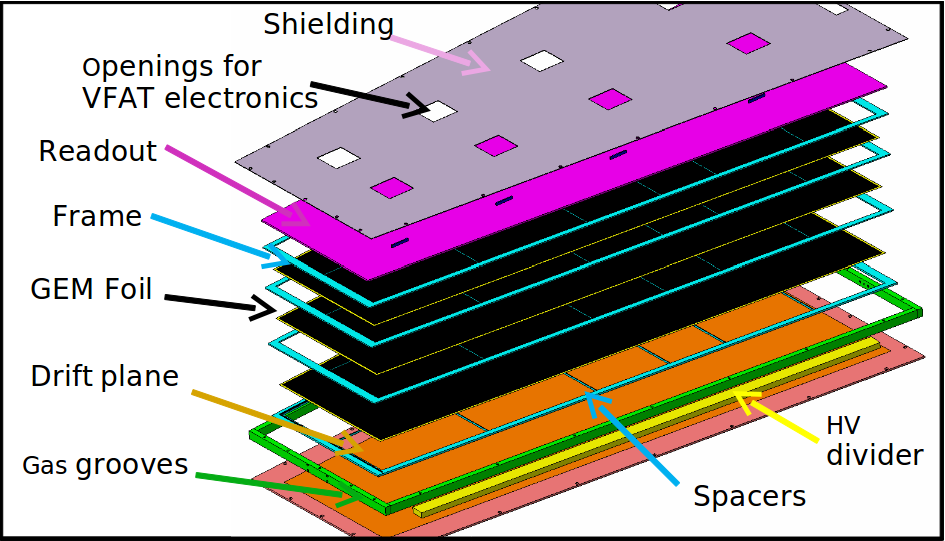
\includegraphics[width=10.0cm,height=7cm]{figures/GEM/ge11cad.png}
		\caption{Layer by layer view of GEM detector}
		\label{ge11}
	\end{center}
\end{figure} 
The trapezoidal chambers are sectorized in $\eta$ partitions to cover $10^0$ each in the azimuthal sector and provide radial readout strip with the strip pointing to the LHC beam pipe (Figure \ref{gemTrapezoidal}). In this design, the strip pitch varies from 0.6 mm (lower side) to 1.2 mm (upper side) with 8-$\eta$ sectors. To improve tracking capabilities, two GEM chambers will be mounted face-to-face to form a double layer called ``Super-Chamber". Thus each Super-Chamber will provide two impact points for each muon track. The gas gap configuration is: 3mm (drift), 1mm (transfer1), 2mm(transfer2), and 1mm (induction) as shown in Figure \ref{tripple-gem}, which proved to be optimal for timing purposes. The gas mixture is $Ar/CO_2/CF_4~45/15/40$.
\begin{figure}[htb]
	\begin{center}
		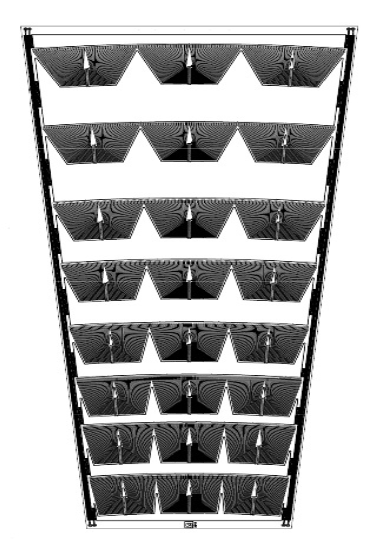
\includegraphics[width=6.0cm,height=12cm]{figures/GEM/gemTrapezoidal.png}
		\caption{Drawing of a large trapezoidal CMS GEM chamber showing $8-\eta$ partitions, each}
		\label{gemTrapezoidal}
	\end{center}
\end{figure} 
\begin{figure}[htb]
	\begin{center}
		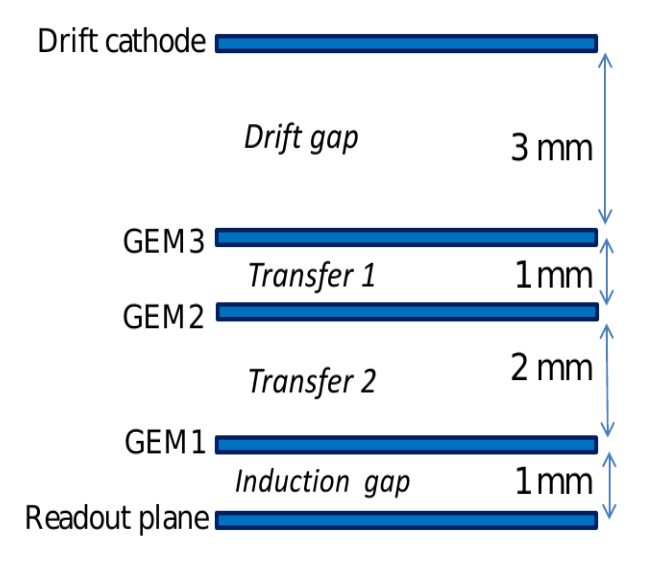
\includegraphics[width=8.0cm,height=6cm]{figures/GEM/tripple-gem.png}
		\caption{Cross-section of the proposed triple-GEM showing the dimensions of the different gaps}
		\label{tripple-gem}
	\end{center}
\end{figure} 
%The GEM production was achieved with the so called "Single-Mask" 
%\subsection{Test beam results}

Two large scale GEM chambers were tested at the SPS H2 beam line at CERN with 150GeV muon/pion beams. A hodoscope of small-area $(10\times 10 cm^2$) double sided GEM chambers was used to predict the hit position in the test chambers (Figure \ref{tbsetup}). Each tracking chamber has, on each side, 256 readout strips with a pitch of 0.4 mm.

\begin{figure}[htb]
	\begin{center}
		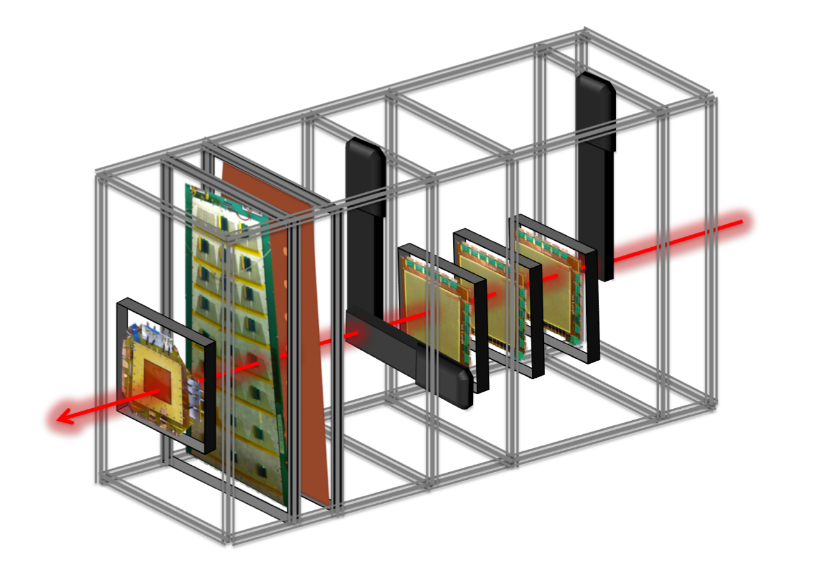
\includegraphics[width=8.0cm,height=6cm]{figures/GEM/tbsetup.png}
		\caption{Schematic view of the test beam setup with the three square GEM hodoscope and the trapezoidal CMS GEM chambers}
		\label{tbsetup}
	\end{center}
\end{figure} 

The full scale CMS GEM chamber has a trapezoidal shape with dimensions of $990\times (220-445)mm$. The strips are segmented in $8-\eta$ partitions. Each partition is sectorized along the $\phi$-coordinate into 3 readout sectors each with 128 strips. Thus 3072 channels are readout for the whole test chamber. During the test beam, two readout scenarios were used: digital TURBO/VFAT2 and Scalable Readout System (SRS) developed by RD51 collaboration and based on APV25 chips. The high voltage powering was realized using a ceramic high voltage divider. The CMS test chamber were placed, closed to the tracking hodoscope, on a vertically movable support to allow scanning. 

%Figure shows teh efficiency obtained
